\documentclass[a4paper, nocolumnsxix]{eskdtext}

%\ESKDtitle{Устройство для получения пчелиного яда}
\ESKDsignature{ВТ.СхТ.КП.П3.16}
\ESKDauthor{Царёв~И.~Г.}
\ESKDchecker{Куцоконь~Н.~С.}
\ESKDcolumnIX{УлГТУ ИВТАПбд-31}

% Настройка стилей для заголовков (запихать внутрь begin если ошибки)
\ESKDsectStyle{section}{\large \bfseries}
\ESKDsectSkip{section}{0pt}{12pt}
\ESKDsectStyle{subsection}{\normalsize \bfseries}
\ESKDsectSkip{subsection}{12pt}{6pt}

%%% Дополнительная работа с математикой
\usepackage{amsmath,amsfonts,amssymb,amsthm,mathtools} % AMS
\usepackage{icomma} % "Умная" запятая: $0,2$ --- число, $0, 2$ --- перечисление

\usepackage{xecyr}
% Enagles loading of OpenType fonts
	\usepackage[cm-default]{fontspec}
\newcommand{\No}{№} % Костыль для совместимости
% Установка глобального шрифта
\setmainfont[Path=/home/ivan/MEGA/Study/Схемотехника/Курсовая работа/Fonts/,
BoldFont=*-bold.ttf,
ItalicFont=*-italic.ttf,
BoldItalicFont=*-bold-italic.ttf,
]{gost-a}

% Нумерация списков цифрами с точкой
\renewcommand{\theenumi}{\arabic{enumi}}
\renewcommand{\labelenumi}{\theenumi.}

\begin{document}
	\itshape
	
	% Создание отдельного стиля для титульника с одной только рамкой
\ESKDnewStyle{Title}{0mm}	
\ESKDputOnStyle{Title}{frame}{\ESKDdrawFrame}
\ESKDthisStyle{Title}

\begin{center}
	\renewcommand{\baselinestretch}{1}
	\small
		Федеральное агентство по образованию \\
		Ульяновский государственный технический университет \\
		Факультет информационных систем и технологий \\
		Кафедра "Вычислительная техника" \\
	
	\normalsize
	\vspace{30ex}
	\renewcommand{\baselinestretch}{1.5}
		Дисциплина: Схемотехника ЭВМ
		
	\renewcommand{\baselinestretch}{1.5}
	\large 
		\textbf{Пояснительная записка к курсовому проекту}
		
		Устройство для получения пчелиного яда
\end{center}

\vspace{20ex}
\begin{flushright}
	Выполнил: \\
	студент группы ИВТАПбд-31 \\
	Царёв И.Г. \\
	Проверил: \\ 
	старший преподаватель \\
	Куцоконь Н.С.
\end{flushright}

\vfill
\begin{center}
	Ульяновск 2016
\end{center}				% Титульник
	
	\makedocname{Устройство для получения пчелиного яда}{}{1}
	\ESKDthisStyle{formII}				% Стиль Форма 2 для оглавления
		\tableofcontents				% Оглавление	
		
	\section{Задание}
Цель курсового проекта состоит в следующем: 
\begin{enumerate}
	\item Систематизировать, закрепить и расширить теоретические знания, полученные по дисциплине "Схемотехника"; 
	\item Привить навыки самостоятельного использования полученных в процессе обучения знаний; 
	\item Приобрести опыт в проектировании и анализе цифровых и цифро-аналоговых узлов и устройств; 
	\item Расширить кругозор в области цифровой вычислительной техники; 
	\item Получить практические навыки в оформлении конструкторской документации. 
\end{enumerate}

В курсовом проекте для рассматриваемого устройства, в данном случае речевого сигнализатора, требуется выполнить следующее: 

\begin{enumerate}
		\item Изложить принцип работы устройства; 
		\item Построить структурную схему устройства; 
		\item Построить полную функциональную схему устройства; 
		\item Построить принципиальную схему устройства; 
		\item Дать временные диаграммы работы устройства; 
		\item Привести спецификацию элементной базы устройства; 
		\item Дать расчет технических характеристик устройства; 
		\item Указать пути совершенствования и модификации устройства.
\end{enumerate}
				% Задание
	\likechapter{ВВЕДЕНИЕ}

Задача обнаружения сигналов на~фоне помех остается одной из~важнейших задач цифровой обработки сигналов и~является актуальной во многих прикладных областях. 
				% Введение
	\section{История вопроса}

В настоящее время известно много устройств для сбора пчелиного яда. По принципу раздражения пчел они разделяются на механические и электрические.

\subsection*{Механический способ}

Большинство модификаций механического способа раздражения пчел для взятия ядовитого секрета сопровождается гибелью пчел. Для получения яда живые пчелы берутся пинцетом или пальцами, жало при этом высовывается наружу. Тонким глазным пинцетом оно слегка извлекается из камеры, после чего начинается автомати­ческое истечение яда. Кончиком жала прикасаются к поверхности стекла, яд изливается на него и быстро засыхает.

Все устройства, основанные на механическом принципе раздра­жения пчел, имеют ряд существенных недостатков:
\begin{enumerate}
	\item В большинстве устройств и приспособлений для сбора яда пчелы гибнут из-за отрыва ядовитой железы; 
	\item Крайне низкая эффективность устройств, осложненная высо­кой трудоемкостью процесса;
	\item Сбор яда в жидкую среду, где он нестоек, быстро подвергает­ся бактериальному распаду и теряет активность (Артемов Н. М., 1969);
	\item Высокая вероятность поражения (ужаления) пчелами обслужи­вающего персонала.
\end{enumerate}

\subsection*{Электрический способ}

Подлинный переворот в технологии получения пчелиного яда произошел, когда в качестве раздражителя был применен электрический ток. Дело в том, что в основе всех рефлекторных физиологических реакций организма человека и животных лежат электрические, точнее \longndash биоэлектрические процессы, то есть метод электрического раздражения удобен тем, что электрический импульс, наносимый на живую ткань извне, будет адекватным, физиологическим раздражителем. Можно подобрать сигнал такой величины и формы, чтобы он вызвал раздражение, приводящее к ужалению, но не был бы опасен для жизнедеятельности пчелы.

Современный комплекс аппаратуры для получения пчелиного яда включает два основных компонента \longndash электрический стимулятор и ядоприёмник.

Электрический стимулятор представляет собой генератор импульсов тока определенной величины и формы.

Ядоприемник является вторым неотъемлемым компонентом комплекса и представляет собой систему близко расположенных между собой проводов-электродов, через которые импульсы со стимулятора доводятся до тела (конечностей) пчелы. Под проводами-электродами обычно находится стекло \longndash собственно ядоприёмник (см. рисунок. \ref{img:poison_reciever}). Пчела, находящаяся на проводах-электродах, замыкает их в цепь и принимает удар импульсного тока. Возникающая при этом реакция ужаления приводит к тому, что с выдвинутого из брюшка пчелы жала стекает ядовитый секрет, который при высыхании и представляет собой сухой пчелиный яд.

\begin{figure}[h]
  \center{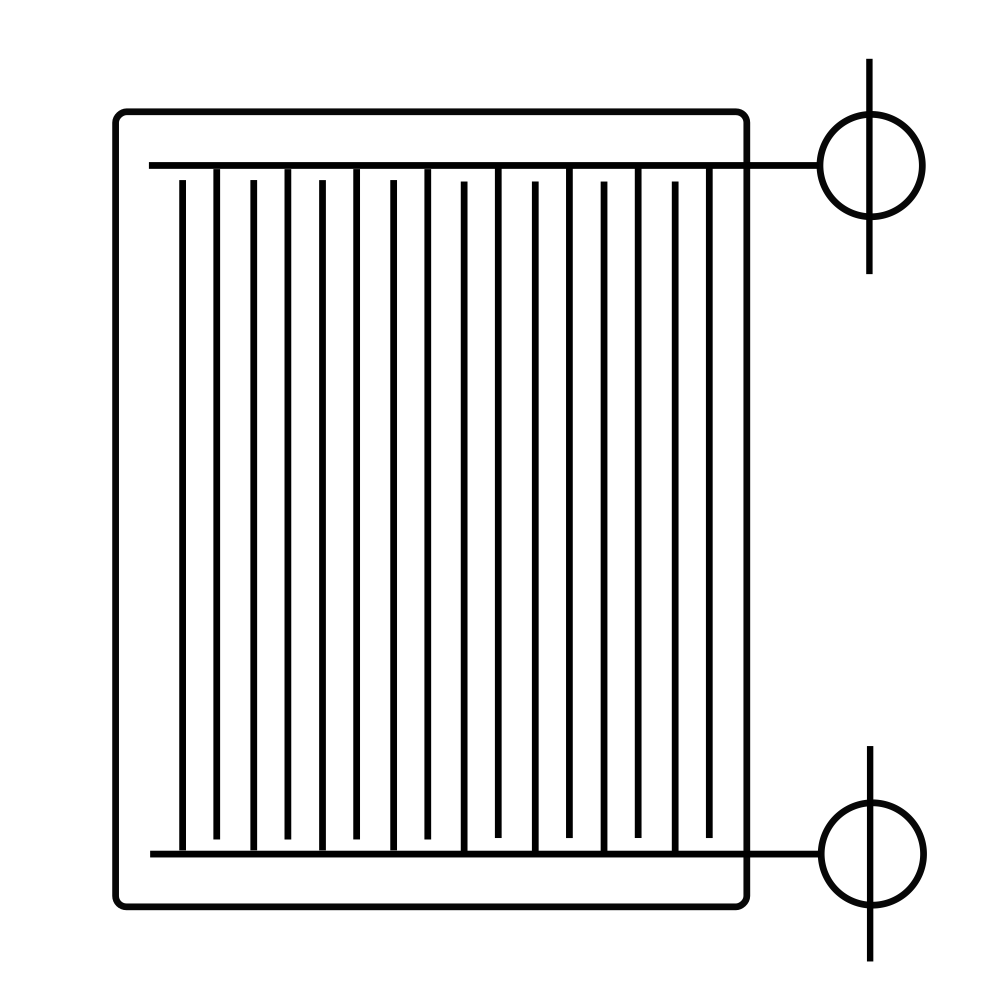
\includegraphics[width=0.25\textwidth]{Images/poison_reciever_scheme.png}}
  
  \caption{Схематичное представление ядоприемника}
  \label{img:poison_reciever}
\end{figure}

\subsection*{Биологическая составляющая}

Пчела, как и другие животные, имеет центральную и периферическую нервную системы, мышцы, которыми эти системы управляют. Управляющие команды нервной системы регулируются сигналами, приходящими по чувствительным нервным путям от рецепторов, находящихся повсеместно \longndash внутри и на поверхности организма.

Рассмотрим пример. Если несильно надавить на тело пчелы, она будет поднимать лапки, крылья. Если давление усилить \longndash пчела попытается улететь. Наконец, сильное надавливание приведет к попытке ужалить. Следовательно, эти инстинктивные рефлексы и соответствующие реакции градуальны и зависят от раздражающего действия, то есть пчела будет жалить только при достижении определенной, пороговой силы раздражителя.

Установлено, что оптимальным будет раздражение, наносимое в режиме импульсов, причем частота этих импульсов должна соответствовать физиологической частоте. Опытным путем определено, что оптимальная частота электрических импульсов раздражения пчел должна лежать в интервале 500-1000 Гц[Крылов, пчелиный яд].

Стоит заметить, что чем медленнее нарастает величина электрического раздражителя, тем выше становится порог, при котором возникает реакция на раздражение (явление аккомодации). Наоборот, мгновенно нарастающий стимул вызовет реакцию ткани при меньшей величине. Поэтому наиболее эффективны электростимуляторы, у которых передний фронт (крутизна) импульса наиболее короток (0,5-1 мс) \longndash генераторы прямоугольных импульсов.

Важным фактом является то, чтобы получить ответную реакцию пчелы на раздражение, нужно подать пачку импульсов, а не одиночный импульс. Поскольку, при одиночном стимуле даже большой силы мышца отвечает одиночным сокращением.

С другой стороны, для полного выброса яда из мышечного резервуара, мышцы его стенок должны работать в режиме насоса \longndash переодическом сокращении и ослаблении. Соответственно должны быть предусмотрены паузы между пачками импульсов.

Как утверждает автор в [крылов пчелиный яд], в условиях пасеки было подтверждено, что при вышеуказанных параметрах длительности и формы импульсов оптимальная амплитуда составила 25-35 В. При достижении величины в 80 В происходит гибель пчёл на электродах. Также было подтверждено, что повышение амплитуды импульсного тока выше 35 В не приводило к дальнейшему увеличению ядоотдачи.		% История вопроса
%	\section{Принцип работы}

Выше было отмечено, что устройство должно работать на пасеке при отсутствии электросети, т. е. должно быть автономным. Принимая также во внимание рассмотренные биологические особенности пчёл, устройство представляет собой электронную систему с ядоприёмником, структурная схема которой представлена на стр.~\pageref{Structural}.

Первичным источником питания в устройстве является автомобильный аккумулятор, к которому подключены ШИМ-регулятор и стабилизатор напряжения. Стабилизатор позволяет получить напряжение величиной +9~В для питания микросхем устройства, а ШИМ-регулятор формирует напряжение, изменяемое в диапазоне от +5 до +12 В, для обеспечения возможности подстройки напряжения на электродах ядоприёмника.

С помощью ключа SA1 устройство можно запустить с задержкой, а с помощью кнопки SB1 \longndash без задержки. Отличие режимов заключается в том, что в первом случае начинает работать генератор импульса запуска, формирующий импульсы с периодом следования 28 часов. В таком случае задержка составляет половину этого периода. Импульс запуска переводит выход триггера в состояние высокого логического уровня, который запускает генератор импульса остановки с периодом следования 1 час.

В то же время триггер запускает мультивибратор и генератор прямоугольных импульсов с регулируемой частотой и скважностью, который модулирует работу мультивибратора, формируя тем самым пачки импульсов частотой 1 кГц. Мультивибратор управляет двумя транзисторными ключами, которые попеременно коммутируют постоянное напряжение, поступающее с ШИМ-регулятора на первичную обмотку трансформатора. Это позволяет получить переменное напряжение прямоугольной формы.

Для повышения полученного переменного напряжения до нужной величины служит повышающий трансформатор, напряжение со вторичной обмотки которого подаётся на электроды ядоприёмника.



	% Принцип работы
	\ESKDthisStyle{formII}	
		\section{Структурная схема}
\makedocname{Устройство для получения пчелиного яда}{Схема структурная}{0}
\begin{figure}
 \centering
 \includepdf[scale=0.7,pages=1, angle=90]{Images/Structural.pdf}
\end{figure}
	% Структурная схема
	\ESKDthisStyle{formII}
		\section{Функциональная схема}
\begin{figure}
 \centering
 \includepdf[scale=0.7,pages=1, angle=-90]{Images/Функциональная.pdf}
\end{figure}	% Функциональная схема
	\ESKDthisStyle{formII}
		\section{Принципиальная схема}
\makedocname{Устройство для получения пчелиного яда}{Схема электрическая принципиальная}{0}
\begin{figure}
 \centering
 \includepdf[scale=0.8, offset=25 25, angle=90]{Images/Principal.pdf}
\end{figure}		% Принципиальная схема
%	\section{Описание работы устройства}

Работа схемы начинается в момент подключения источника питания к разъёму XP1. 

Стабилизированное напряжение 9~В через резистор R1 поступает на входы сброса генератора G1 и  счётчика D1, держа их в сброшенном состоянии. Также в момент включения конденсатор C5 оказывается разряженным, поэтому на входе R триггера D4 оказывается логическая единица. Конденсатор начинает заряжаться через резистор R4. По мере заряда потенциал на входе R триггера D4 понижается до уровня логического нуля. Данная цепь R5-C4 позволяет получить на входе R триггера импульс, переводящий прямой выход триггера в состояние логического нуля. Этот сигнал держит в сброшенном состоянии генератор G3, а логическая единица с инверсного выхода \longndash генератор G2 и счётчик D2. Также сигнал с этого выхода поступает на элемент логического И-НЕ D5, на выходе которого формируется логическая единица, которая держит генератор G4 в сброшенном состоянии. Поэтому силовые ключи оказываются закрытыми и на выходе схемы на разъёме XP2 напряжение равно нулю. В данном состоянии схема может находиться сколь угодно долго.

Включение устройства в работу производится замыканием ключа SA1. При этом на входах сброса G1 и D1 появляется логический нуль, разрешающий их работу. По истечению T=T\textsubscript{1}/2 часов на выходе делителя D3 появляется логическая единица. Дифференцирующая цепочка R8-C4 обеспечивает появление импульса логической единицы на входе S триггера. При этом на прямом выходе триггера появляется логическая единица, а на инверсном \longndash логический нуль. Это приводит к тому, что генераторы G2, G3 и счётчик D2 начинают работу. Также логический нуль с инверсного выхода триггера поступает на один из входов D5. В моменты, когда сигнал с генератора G3 имеет низкий логический уровень, происходит изменение сигнала на выходе D5 с низкого на высокий логический уровень. При этом начинат работать генератор G4. Противофазные импульсы на выходах генератора G4 попеременно открывают силовые ключи, которые подключают напряжение с ШИМ-регулятора на первичную обмотку трансформатора T1, вследствие чего на его первичной обмотке возникает переменное напряжение. Далее оно усиливается и поступает на выход XP2.

Формирование переменного напряжения на выходе происходит в течение времени равным T\textsubscript{2}/2 часов. По истечению этого времены, на выходе счётчика D2 возникает логическая единица, которая сбрасывает триггер, изменяя состояние его выходов на противоположные. Это приводит к отключению генератора G2 и G3 и сбросу счётчика D2. Также происходит отключение генератора G4 и, следовательно, напряжение на выходе трансформатора T1 станет равным нулю. Схема возвращается в исходное состояние и ожидает появление следующего переднего фронта импульса с выхода D3.

Следует отметить, что возможно включение схемы без дополнительной задержки путем подачи короткого импульса напрямую на вход S триггера при помощи кнопки SB1.

Для регулировки выходного напряжения в схеме ШИМ-регулятора имеется возможность подстройки его выходного напряжения в небольших пределах при помощь переменного резистора R20.
	% Описание работы устройства
%	\section{Временные диаграммы}

\begin{figure}
 \centering
 \includepdf[scale=0.85, offset=25 -20]{Images/Diagrams.pdf}
\end{figure}
		% Временные диаграммы
%	\section{Описание микросхем}

Приведем перечень некоторых электрических параметров интегральных микросхем, их буквенные обозначения и определения, установленные ГОСТ 19480-74 “Микросхемы интегральные. Электрические параметры. Термины, определения и буквенные обозначения”, ГОСТ 18683-73 “Микросхемы интегральные логические. Методы измерения электрических параметров”, ГОСТ 19799-74 “Микросхемы интегральные аналоговые. Методы измерения электрических параметров и определения характеристик”. Затем по этим параметрам дадим характеристику микросхемам, используемым в схеме устройства, а именно микросхемам:

\begin{itemize}
	\item К1114ЕУ4
	\item К176ИЕ12
	\item К561ТМ2
	\item К176ИЕ5
	\item К561ЛЕ10
	\item К561ЛА7
\end{itemize}

\subsection*{Электрические параметры микросхем}

\textbf{Ток потребления $I_{\text{пот}}$} \longndash значение тока, потребляемого микросхемой от источников питания в заданном режиме. 

\textbf{Ток потребления в состоянии логического нуля $I_{\text{пот}}^{0}$.} 

\textbf{Ток потребления в состоянии логической единицы $I_{\text{пот}}^{1}$.} 

\textbf{Напряжение логического нуля $U_0$} \longndash значение низкого уровня напряжения для “положительной” логики и значение высокого уровня напряжения для “отрицательной” логики. 

\textbf{Напряжение логической единицы $U_1$} – значение высокого уровня напряжения для “положительной” логики и значение низкого уровня напряжения для “отрицательной” логики. 

\textbf{Входной ток логического нуля $I_{\text{вх}}^{0}$.}

\textbf{Входной ток логической единицы $I_{\text{вх}}^{1}$.}

\textbf{Ток утечки на входе $I_{\text{ут,вх}}$} \longndash значение тока во входной цепи микросхемы при закрытом состоянии входа и заданных режимах на остальных выводах.
 
\textbf{Время задержки распространения сигнала при включении $t_{\text{зд,p}}^{1,0}$} \longndash интервал времени между входным и выходным импульсами при переходе напряжения на выходе микросхемы от напряжения логической единицы к напряжению логического нуля, измеренный на уровне 0,5 или на заданных значениях напряжения.

\textbf{Время задержки распространения сигнала при выключении  $t_{\text{зд,p}}^{0,1}$} \longndash интервал времени между входным и выходным импульсами при переходе напряжения на выходе микросхемы от напряжения логического нуля к напряжению логической единицы, измеренный на уровне 0,5 или на заданных значениях напряжения. 

\textbf{Помехоустойчивость статическая $U_{\text{п,ст}}$} \longndash наибольшее значение допустимого напряжения статической помехи по высокому и низкому уровням входного напряжения, при котором еще не происходит изменение уровней выходного напряжения цифровой интегральной микросхемы. 

\textbf{Коэффициент разветвления по выходу $K_{\text{раз}}$} \longndash число единичных нагрузок, которое можно одновременно подключить к выходу микросхемы (единичной нагрузкой является один вход основного логического элемента данной серии интегральных микросхем).

\subsection*{К1114ЕУ4}

Микросхема представляет собой многофункциональную схему управления источником вторичного электропитания (двухтактный ШИМ-контроллер). ИС осуществляет формирование опорного напряжения, усиление сигнала ошибки, формирование пилообразного напряжения, ШИМ-модуляцию, формирование 2-тактного выхода, защиту сквозных токов, защиту от перегрузок, включение и выключение, внешнюю синхронизацию, формирование частотной характеристики и обеспечение мягкого запуска. Корпус типа 238.16-2, масса не более 1,5 г.

\begin{figure}[ht]
  \center{\includegraphics[width=0.5\textwidth]{Images/К1114ЕУ4.png}}
  
  \caption{Условно-графическое обозначение К1114ЕУ4}
  \label{img:k1114eu4}
\end{figure}

Назначение выводов:
1 \longndash неинвертирующий вход $\text{ОУ} 1$;
2 \longndash интвертирующий вход $\text{ОУ} 1$;
3 \longndash выход усилителей;
4 \longndash установка паузы;
5 \longndash вход для подключения конденсатора задания частоты;
6 \longndash вход для подключения резистора задания частоты;
7 \longndash общий;
8 \longndash коллектор $VT1$;
9 \longndash эмиттер $VT1$;
10 \longndash эмиттер $VT2$;
11 \longndash коллектор $VT2$;
12 \longndash напряжение питания;
13 \longndash блокировка двухтактного выхода;
14 \longndash выход источника опорного напряжения;
15 \longndash инвертирующий вход ОУ 2;
16 \longndash неинвертирующий вход ОУ 2; 

\subsection*{К176ИЕ12}

Микросхема представляет собой двоичный счётчик на 60 и 15-разрядный делитель частоты. Содержит 696 интегральных элементов. Корпус типа 238.16-1 и типа 2103.16-11, масса не более 1,5 г. \\

\begin{figure}[ht]
  \center{\includegraphics[width=0.3\textwidth]{Images/К176ИЕ12.png}}
  
  \caption{Условно-графическое обозначение К176ИЕ12}
  \label{img:k176ie12}
\end{figure}

Назначение выводов: 1 \longndash выход мультиплексора $(2^6)$, T2; 2 \longndash выход мультиплексора $(2^3)$, T4; 3 \longndash выход мультиплексора $(2^6)$, T1; 4 \longndash выход делителя $(2^{15})$; 5 \longndash вход установка "0" делителя R1; 6 \longndash выход делителя $(2^{14})$; 7 \longndash вход счётчика C2; 8 \longndash общий; 9 \longndash вход установка "0" счётчика, R2; 10 \longndash выход счётчика; 11 \longndash выход делителя $(2^5)$; 12 \longndash вход делителя C1; 13 \longndash выход делителя (=) инверсный; 14, 15 \longndash выходы делителя; 16 \longndash напряжение питания.

\subsubsection*{Электрические параметры}
\begin{itemize}
	\item[] Номинальное напряжение питания \dotfill $9~\text{В} \pm 5\%$
	\item[] Выходное напряжение низкого уровня \dotfill $\leq 0,3~\text{В}$
	\item[] Выходное напряжения высокого уровня \dotfill $\geq 8,2~\text{В}$
	\item[] Входной ток низкого уровня \dotfill $\geq -0,3~\text{мкА}$
	\item[] Входной ток высокого уровня \dotfill $\leq 0,3~\text{мкА}$
	\item[] Ток потребления \dotfill $\leq 25~\text{мкА}$
	\item[] Ток потребления в динамическом режиме \dotfill $\leq 0,3~\text{мА}$
	\item[] Мощность потребления \dotfill $\leq 50~\text{мВт}$
	\item[] Частота тактовых сигналов \dotfill $\geq 1,2~\text{МГц}$
	\item[] Входная емкость \dotfill $\leq 10~\text{пФ}$
	\item[] Коэффициент разветвления по выходу \dotfill $\leq 50$
\end{itemize}

\subsection*{К561ТМ2}

Микросхема представляет собой два D-триггера с динамическим управлением. Установка триггера по входам R и S принудительная, поэтому сигналы синхронизации C и информационного входа D не изменяют состояния триггера на выходе во время действия сигналов R и S. Содержит 128 интегральных элементов. Корпус типа 201.14-1, масса не более 1 г и 4306.14-А.

\begin{figure}[ht]
  \center{\includegraphics[width=0.25\textwidth]{Images/К561ТМ2.png}}
  
  \caption{Условно-графическое обозначение К561ТМ2}
  \label{img:k561tm2}
\end{figure}

Назначение выводов: 1 \longndash выход $Q1$; 2 \longndash выход $\bar{Q1}$; 3 \longndash вход $C1$; 4 \longndash вход $R1$; 5 \longndash вход $D1$; 6 \longndash вход $S1$; 7 \longndash общий; 8 \longndash вход $S2$; 9 \longndash вход $D2$; 10 \longndash вход $R2$; 11 \longndash вход $C2$; 12 \longndash выход $\bar{Q2}$; 13 \longndash выход $Q2$; 14 \longndash напряжение питания.

\begin{figure}[ht]
  \center{\includegraphics[width=0.8\textwidth]{Images/truthtable.png}}
  
  \caption{Таблица истинности К561ТМ2}
  \label{img:truthtable}
\end{figure}

\subsubsection*{Электрические параметры}
\begin{itemize}
    \item[] Напряжение питания \dotfill $3...15~\text{В}$
    \item[] Выходное напряжение низкого уровня при воздействии помехи:
    \begin{itemize}
	    \item[] при $U_{\text{п}}=5~\text{В}$ \dotfill $\leq 0,8~\text{В}$
	    \item[] при $U_{\text{п}}=10~\text{В}$ \dotfill $\leq 1~\text{В}$
    \end{itemize}
    \item[] Выходное напряжения высокого уровня при воздействии помехи: 
    \begin{itemize}
	    \item[] при $U_{\text{п}}=5~\text{В}$ \dotfill $\geq 4,2~\text{В}$ 
	    \item[] при $U_{\text{п}}=10~\text{В}$ \dotfill $\geq 9~\text{В}$
    \end{itemize}
    \item[] Ток потребления при $U_{\text{п}}=15~\text{В}$ \dotfill $\leq 25~\text{мкА}$
    \item[] Входной ток низкого (высокого) уровня при $U_{\text{п}}=15~\text{В}$  \dotfill $\leq -0,3~\text{мкА}$
    \item[] Выходной ток низкого уровня: 
    \begin{itemize}
	    \item[] при $U_{\text{п}}=5~\text{В}$ \dotfill $\geq 0,5~\text{мА}$ 
	    \item[] при $U_{\text{п}}=10~\text{В}$ \dotfill $\geq 0,9~\text{мА}$
    \end{itemize}
    \item[] Выходной ток высокого уровня: 
    \begin{itemize}
	    \item[] при $U_{\text{п}}=5~\text{В}$ \dotfill $\geq 0,25~\text{мА}$ 
	    \item[] при $U_{\text{п}}=10~\text{В}$ \dotfill $\geq 0,6~\text{мА}$
    \end{itemize}
    \item[] Время задержки распространения при включении (выключении): 
    \begin{itemize}
	    \item[] при $U_{\text{п}}=5~\text{В}$ \dotfill $\leq 420~\text{нс}$ 
	    \item[] при $U_{\text{п}}=10~\text{В}$ \dotfill $\leq 150~\text{нс}$
    \end{itemize}
    \item[] Входная емкость при $U_{\text{п}}=10~\text{В}$ \dotfill $\leq 10~\text{пФ}$
\end{itemize}


\subsection*{К176ИЕ5}

Микросхема представляет собой 15-разрядный двоичный делитель частоты. Содержит 307 интегральных элементов. Корпус типа 2102.14-4 и типа 201.14-1, масса не более 1 г.

\begin{figure}[ht]
  \center{\includegraphics[width=0.3\textwidth]{Images/К176ИЕ5.png}}
  
  \caption{Условно-графическое обозначение К176ИЕ5}
  \label{img:k176ie5}
\end{figure}

Назначение выводов: 1 \longndash выход 9 разряда; 2 \longndash выход 10 разряда; 3 \longndash вход установки "0" R; 4 \longndash выход 14 разряда; 5 \longndash выход 15 разряда; 6,7 \longndash общие; 8, 13 \longndash свободные; 9 \longndash вход $T$; 10 \longndash выход $\bar{T}$; 11 \longndash выход $\bar{A}$; 12 \longndash выход $A$; 14 \longndash напряжение питания.

\subsubsection*{Электрические параметры}
\begin{itemize}
	\item[] Номинальное напряжение питания \dotfill $9~\text{В} \pm 5\%$
	\item[] Выходное напряжение низкого уровня \dotfill $\leq 0,3~\text{В}$
	\item[] Выходное напряжения высокого уровня \dotfill $\geq 8,2~\text{В}$
	\item[] Входной ток низкого уровня \dotfill $\geq -0,5~\text{мкА}$
	\item[] Входной ток высокого уровня \dotfill $\leq 0,5~\text{мкА}$
	\item[] Ток потребления \dotfill $\leq 0,25~\text{мкА}$
	\item[] Ток потребления в динамическом режиме \dotfill $\leq 0,3~\text{мА}$
	\item[] Максимальная мощность \dotfill $\leq 21~\text{мВт}$
	\item[] Тактовая частота деления \dotfill $\geq 1~\text{МГц}$
	\item[] Нагрузочная способность в статическом режиме \dotfill $\leq 15$
\end{itemize}

\subsection*{К561ЛЕ10}

Микросхема представляет собой три трехвходовых элемента ИЛИ-НЕ. Содержат 54 интегральных элемента. Корпус типа 201.14-1, масса не более 1 г, и 4306.14-А.

\begin{figure}[ht]
  \center{\includegraphics[width=0.2\textwidth]{Images/К561ЛЕ10.png}}
  
  \caption{Условно-графическое обозначение К561ЛЕ10}
  \label{img:k561le10}
\end{figure}

Назначение выводов: 1,2,3,4,5,7,11,12,13 \longndash входы; 6,9,10 \longndash выходы; 7 \longndash общий; 14 \longndash напряжение питания.

\subsubsection*{Электрические параметры}
\begin{itemize}
	\item[] Напряжение питания \dotfill $3...15~\text{В}$
	\item[] Выходное напряжение низкого уровня \dotfill $\leq 0,01~\text{В}$
	\item[] Максимальное выходное напряжения низкого уровня \dotfill $\leq 2,9~\text{В}$
	\item[] Минимальное выходное напряжения высокого уровня \dotfill $\geq 7,2~\text{В}$
	\item[] Ток потребления \dotfill $\leq 5~\text{мкА}$
	\item[] Входной ток низкого уровня \dotfill $\leq|-0,05|~\text{мкА}$
	\item[] Входной ток высокого уровня \dotfill $\leq 0,05~\text{мкА}$
	\item[] Выходной ток низкого уровня \dotfill $\geq 0,6~\text{мА}$
	\item[] Выходной ток высокого уровня \dotfill $\geq|-0,25|~\text{мА}$
	\item[] Ток потребления в динамическом режиме \dotfill $\leq 0,3~\text{мА}$
	\item[] Время задержки распр. входного сигнала при включении \dotfill $\leq 125~\text{нс}$
	\item[] Время задержки распр. входного сигнала при выключении \dotfill $\leq 145~\text{нс}$
\end{itemize}

\subsection*{К561ЛА7}

Микросхема представляет собой четыре логических элемента 2И-НЕ. Содержат 64 интегральных элемента. Корпус типа 201.14-1, масса не более 1 г и 4306.14-А.

\begin{figure}[ht]
  \center{\includegraphics[width=0.2\textwidth]{Images/К561ЛА7.png}}
  
  \caption{Условно-графическое обозначение К561ЛА7}
  \label{img:k561la7}
\end{figure}

Назначение выводов: 1 \longndash вход $X2$; 2 \longndash вход $X1$; 3 \longndash выход $Y1$; 4 \longndash выход $Y2$; 5 \longndash вход $X3$; 6 \longndash вход $X4$; 7 \longndash общий; \longndash вход $X6$; 9 \longndash вход $X5$; 10 \longndash выход $Y3$; 11 \longndash выход $Y4$; 12 \longndash вход $X7$; 13 \longndash вход $X8$; 14 \longndash напряжение питания.

\subsubsection*{Электрические параметры}
\begin{itemize}
    \item[] Напряжение питания \dotfill $3...15~\text{В}$
    \item[] Выходное напряжение низкого уровня при воздействии помехи:
    \begin{itemize}
	    \item[] при $U_{\text{п}}=10~\text{В}$ \dotfill $\leq 2,9~\text{В}$
	    \item[] при $U_{\text{п}}=5~\text{В}$ \dotfill $\leq 0,95~\text{В}$
    \end{itemize}
    \item[] Выходное напряжения высокого уровня при воздействии помехи при $U_{\text{п}}=10~\text{В}$ \dotfill $\geq 7,2~\text{В}$
    \item[] Ток потребления при $U_{\text{п}}=15~\text{В}$ \dotfill $\leq 5~\text{мкА}$
    \item[] Входной ток низкого (высокого) уровня при $U_{\text{п}}=15~\text{В}$  \dotfill $\leq -0,3~\text{мкА}$
    \item[] Выходной ток низкого уровня: 
    \begin{itemize}
	    \item[] при $U_{\text{п}}=10~\text{В}$ \dotfill $\geq 1,3~\text{мА}$ 
	    \item[] при $U_{\text{п}}=5~\text{В}$ \dotfill $\geq 0,51~\text{мА}$
    \end{itemize}
    \item[] Выходной ток высокого уровня: 
    \begin{itemize}
	    \item[] при $U_{\text{п}}=10~\text{В}$ \dotfill $\geq 1,3~\text{мА}$ 
	    \item[] при $U_{\text{п}}=5~\text{В}; U_{\text{вых}}=4,6~\text{В}$ \dotfill $\geq 0,51~\text{мА}$
	    \item[] при $U_{\text{п}}=5~\text{В}; U_{\text{вых}}=2,5~\text{В}$ \dotfill $\geq 1,6~\text{мА}$
    \end{itemize}
    \item[] Время задержки распространения при включении (выключении): 
    \begin{itemize}
	    \item[] при $U_{\text{п}}=10~\text{В}$ \dotfill $\leq 80~\text{нс}$ 
	    \item[] при $U_{\text{п}}=5~\text{В}$ \dotfill $\leq 160~\text{нс}$
    \end{itemize}
    \item[] Входная емкость \dotfill $\leq 11~\text{пФ}$
\end{itemize}	% Описание микросхем
%	\chapter{Расчётная часть}
\section{Безыдентификационная псевдоградиентная адаптация}
Суть псевдоградиентной процедуры применительно к~поставленной задаче в~следующем. На каждой итерации вычисляются оценки параметров привязки в~соответствии с~выражением
\[
\hat{\bar{\alpha}}_{t+1}=\hat{\bar{\alpha}}_{t}-\Lambda_{t}\bar{\beta}_{t}
\]
где: $\bar{\alpha}$ -- \textit{m}-мерный вектор оцениваемых параметров, $t=\overline{0,T}$ -- номер итерации, $\Lambda_{t}$ -- матрица усиления (всегда положительно определенная матрица, как правило диагональная, что исключает собственно матричные вычисления), $\bar{\beta}_{t}$ -- псевдоградиент целевой функции $J(\bar{\alpha})$ (случайный вектор, зависящий в~общем случае от~$\bar{\alpha}_{t-1}$ и~целевой функции $J(\bar{\alpha})$).

Для нестационарных сигналов значения элементов $\lambda_{t}$, $t=\overline{1,T}$, приходится ограничивать снизу для обеспечения вариабельности оценок. Хорошие результаты сходимости оценок можно получить уже при использовании знаковой функции от~значения псевдоградиента на~каждой итерации:
\[
\hat{\bar{\alpha}}_{t+1}=\hat{\bar{\alpha}}_{t}-\Lambda_{t}\text{sign}(\bar{\beta}_{t}),
\]
где
\[
\text{sign}(\beta_{it})= 
\left\{
	\begin{aligned}
		1, &\text{ если } \beta_{it} > 0, \\
		0, &\text{ если } \beta_{it} = 0, \\
		-1, &\text{ если } \beta_{it} < 0, \\
	\end{aligned}
\right.
\]
что значительно упрощает практическую реализацию. 			% Расчётная часть
%	\section{Заключение}

Представленная схема устройства для получения пчелиного яда имеет ряд недостатков, поэтому  возможно её дальнейшее совершенствование.

Устройство собрано на устаревших комплектующих. В настоящее время рациональнее будет использовать для решения поставленной задачи микроконтроллер. Это позволит очень гибко управлять работой прибора:
устанавливать любые интервалы задержки и времени работы, параметров формирования пачек импульсов, а также частоту самих импульсов. Кроме этого станет возможным изменять вышеуказанные параметры автоматически в процессе работы устройства.

Применение микроконтроллера также даёт возможность владельцу удалённо управлять работой устройства и отслеживать текущие настройки.
			% Заключение
	\renewcommand{\refname}{ЛИТЕРАТУРА} \renewcommand{\bibname}{ЛИТЕРАТУРА} 

\begin{thebibliography}{99}
    \addcontentsline{toc}{likechapter}{\refname}
    	
    \vspace{\baselineskip}
	\bibitem{Akimov_1984}Теория обнаружения сигналов / П.С. Акимов, П.А. Бакут, В.А. Богданович и др.: Под редакцией П.А. Бакута. -- М: Радио и связь, 1984 -- 440 с.
	
\end{thebibliography}
		% Список литературы
	
%	%\section{Спецификация}

В~диссертации разработаны алгоритмы работы и~структура системы обнаружения радиоимпульсов и~измерения их основных параметров. 
		% Спецификация
\end{document}